\section{Beginning}\label{sec:beginning}

\begin{wrapfigure}{R}{0.3\textwidth}
    \centering
    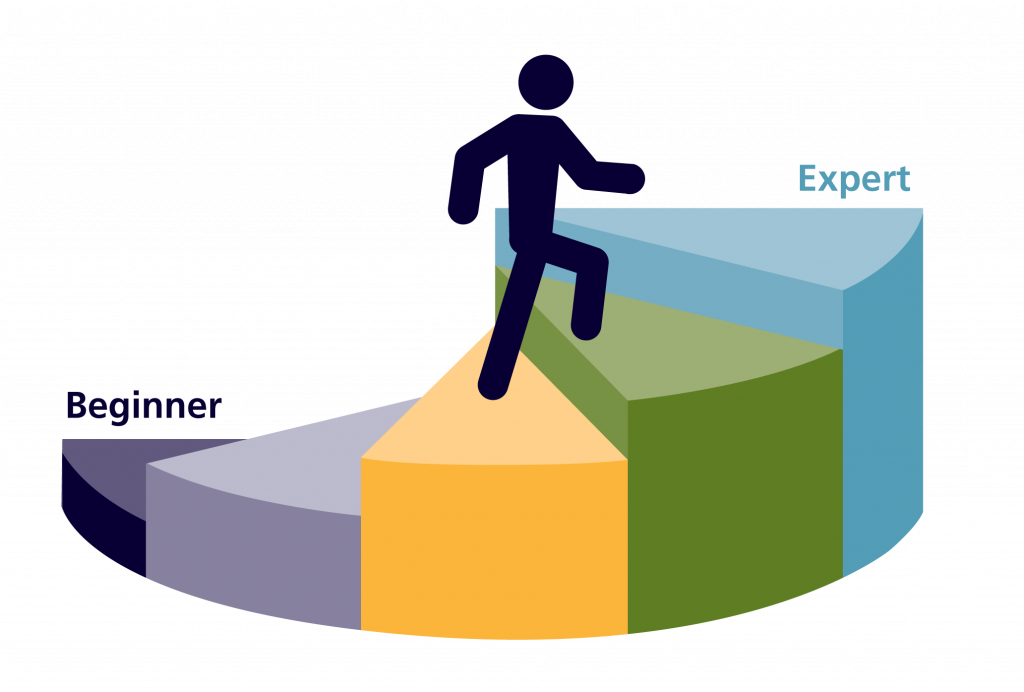
\includegraphics[width=0.25\textwidth]{images/beginning}
\end{wrapfigure}

As a beginner, it can be difficult to get the necessary information to decide whether this art is something for you.
You need to figure out what it actually is, and whether it actually fits you in your needs and also in regard to the physical requirements on the body.
But also more practical aspects like where and how to find a school, how to find a (good) teacher, and what to look out for when doing so.
This section should provide you with some initial directions for taking your first steps into the wonderful world of CI\@.

\subsection{Starting Point}\label{subsec:starting-point}

To start it's always nice to check some \textbf{videos} (see the Resources chapter at the end of this book), but please don't be intimidated right away from what you are seeing.
The people you will see on those videos are usually already on a very high level, and that's not what you are going to encounter at first.

Join a \textbf{recommended teacher} and go first to some classes (see ``How to spot a good teacher'' further below).
It is not advisable to immediately go to jams, but only after 10--20 classes, to already have the basic principles embodied.
And don't give up if your very first experience seems bad; maybe you want to just try another class or another teacher.
Be also aware that CI is not only physical, so ask yourself: Why and what are you doing?
This will be very beneficial and inspiring for your first steps with CI\@.

\subsection{Requirements}\label{subsec:requirements}

You might ask yourself for whom is CI fitted?
For whom is it a good idea to join, or not to join?
Are there any physical requirements and how to deal with if you feel a bit touch-averse towards strangers?

In general, it can be said that every body is welcome, but not necessarily every behaviour.
This art-form is not only for the young and well-trained, as there is no real requirement for acrobatic performance; the body just needs to be mobile and the bones bear some weight.
It is not about \textbf{age}, neither about body ability; yet some techniques might not be possible to do, or would need some adaption.
Students even with the age of 70 would be able to do shoulder lifts, and that person was doing it for many years.
Some of the more crazy things, he mentioned, was better to keep for ``the next life'' though.

Sharing weight, being in contact with another body, exploring what's happening at the moment, where the weight is, the unconscious reaction to balance, \ldots this, anybody can do.
Even with a partially disabled body, with some \textbf{physical disability} like being in a wheelchair, it is possible to play together with a physically fit person.
Or also with blind people, as they are often also super in tune with weight and different other aspects of perception.
It leads to a very different and interesting kind of exploration, and requires us to renegotiate, to re-explore what kind of communication we can play with.

Even with a huge \textbf{weight} difference, we just need to be more careful about which kinds of lifts to do, and who is carrying whom how.
We need to negotiate what's possible, and sometimes this means no shoulder lifts, and/or no rolling over.
Always respect the abilities of the dance and both bodies by checking each other out, slowly (!) and step-by-step, then it becomes \textit{safer}, yet not necessarily \textit{safe}!
When you are about to engage in more advanced (crazy/dangerous) techniques, always do it with a lot of care and a \gls{guardianangel} who will spot you.

In theory, in an ideal world, everyone is welcome, yet it is not advised for people with severe \textbf{touch aversion} to jump into CI, as a solution to their trauma in that field.
It is recommended to better ``tippie toe'' in different kind of forms first, and only then see if they want to continue with CI\@.
Mental challenges sometimes make people join only one (or even half a) class, or sometimes the teacher might even have doubts and expresses that discreetly.
People who take too many risks (the ``dangerous ones''), which are throwing themselves on unknown partners, won't be denied access to classes or jams, but dancers will most likely get aware of that and keep their distance to them, as it won't feel safe.

\subsection{Good Teacher}\label{subsec:good-teacher}

Finding the right teacher is special.
Don’t expect that it will work right from the beginning at the first attempt.
Take your time, have patience.

There are three realms to consider:

\begin{enumerate}
    \item The \textbf{physical} aspect:
    \begin{itemize}
        \item The teacher knows what he is teaching, and also being honest about his limitations in that knowledge; or simply put: \textbf{humbleness}.
        How does he deal with his own weaknesses, flaws and mistakes?
        Is he able to admit to not knowing something, to be mistaken, or simply, which is very human, to have messed up something?
        \item What is his educational \textbf{background}, and for how long is he doing (teaching) it?
        Try to look him up on the internet, maybe there are even some videos from him.
    \end{itemize}
    \item The \textbf{psychological} aspect:
    \begin{itemize}
        \item This includes the ability to \textbf{hold space}, in case when internal processes might happen.
        \item Are common rules laid out transparently and are they comprehensible and challengeable?
        \item \textbf{Safety} is created by the nature of his intention: Does he want to inflate his ego, making himself bigger?
		What happens if doubt is expressed, or if he is criticized in front of others?
        Does he claim to have a status of a master or guru, or is he ``one of us'' and going for a drink with the students, taking off his teacher's hat.
        \item Does he want to gain something from you outside the class, besides monetary compensation in a formally agreed transaction?
        Are personal services and favors expected or even demanded, when you are in individual contact with the teacher?
        \item Contact him personally.
        As long as you are not intrusive and stay respectful, a clear, friendly and in-time response to your questions should be possible.
    \end{itemize}
    \item The \textbf{spiritual} aspect:
    \begin{itemize}
        \item Watch out for the presence of \textbf{competition}.
        Does he genuinely want the student to be as good or even better as himself?
        Basically, does he have a pure intention to teach, sharing his knowledge (whereas this sharing is also always happening two-way though).
        \item It is a good sign if your teacher motivates you to also have a look at other teachers.
    \end{itemize}
\end{enumerate}

\subsection{Becoming Good}\label{subsec:becoming-good}

What makes a good CI practitioner good can be answered in many different ways.
It is for sure not only the obviously physical/technical aspect, but also having the right intention for the dance, a proper attitude and mindset which is led by \textbf{curiosity} -- the antidote to being judgmental.
An advanced practitioner is really happy exploring the smallest thing, being able to keep a beginner's mind open, and he knows what he knows, and he especially also knows what he doesn't know.

For many, dancing with total beginners and total advanced is most enjoyable as they show and remind us the different aspects of the dance.
Both of them are usually very happy to dance with each other as well.
On the other hand, intermediates are usually not happy to dance with beginners; they prefer to only stay with their own level or higher.
They are also usually the ``dangerous ones'', as they know the pathways and the tricks, the form and the looks, but they don't know what they don't know.
They are lacking the listening ability.
If something happens which was not predicted in their pathways, like quick changes, they don't know how to handle that.
They also often go faster than their level of attention, and especially very often go faster than their beginner-partner's level of attention.
Having that said: Always \textbf{respect} what your body is able to do in regard to level, age, and constitution.

A very important tool you must gain in order to get good is the ability to \textbf{listen} to small and subtle sensations in the body, the change of movement and weight.
An increased awareness of incoming information, inside as well as outside the body via the peripheral nervous system, the so-called \gls{skinesphere}.
It leads us to be able to detect what's going on, thus becoming ``well-informed'' and leading us to become a much better dancer.

More generally speaking, we can state that the following personality aspects lead to becoming good (those apply of course also to any other form or practice):

\begin{itemize*}
    \item [] \textbf{Kindness}: Smile, be gentle and soft, with yourself and others.
    \item [] \textbf{Patience}: Let beginners do their own mistakes, gaining experience.
    \item [] \textbf{Humbleness}: By not showing off how many years you are doing this-or-that, and not arrogantly teaching beginners.
\end{itemize*}

Everybody learns and everybody teaches; everybody is a student and teacher at the same time.
There are no certificates.
If you have a lot of knowledge, you will share that by your dancing.

Years of practice itself are not even necessarily a guarantee for expertise or even mastery.
Some people get stuck at a certain level; even after many, many years.
Lots of experience itself doesn't mean your level of technical practise is going forward.
Always keep a \textbf{beginner's mind}: Keep on doing the very same thing, like lifts and spirals, yet stay with curiosity and explore deeper, like the small things and changes, where to focus now, to put your attention and intention to.
Even if someone's technical level is very advanced: The moment where you stop posing questions, is where you stop developing.